%----------------------------------------------------------------------------------------
%	PACKAGES AND DOCUMENT CONFIGURATIONS
%----------------------------------------------------------------------------------------

\documentclass{article}


\usepackage{graphicx} % Required for the inclusion of images
\graphicspath{{figures/}}
\usepackage{subfigure} % Required for the inclusion of images
\usepackage{natbib} % Required to change bibliography style to APA
\usepackage{amsmath} % Required for some math elements 
\usepackage{listings}
\usepackage{xcolor}
\usepackage{fontspec}
%\usepackage{ctex}
\setmonofont{Consolas}
\lstset{
basicstyle=\ttfamily\scriptsize,%
escapeinside=``,%
keywordstyle=\color{black},%\bfseries, \underbar,%
identifierstyle={},%
commentstyle=\color{black},%
stringstyle=\ttfamily,%
%labelstyle=\tiny,%
extendedchars=false,%
linewidth=\textwidth,%
numbers=left,%
numberstyle=\tiny \color{blue},%
frame=trbl%
}


%\usepackage{times} % Uncomment to use the Times New Roman font

%----------------------------------------------------------------------------------------
%	DOCUMENT INFORMATION
%----------------------------------------------------------------------------------------

\title{\textbf{Project 1: Optimizing the Performance of a Pipelined Processor}} % Title

\author{519021910095, QianyunGuo, guoqianyun@sjtu.edu.cn \\
        519021910575 , MuchenPan, pmc296289396@sjtu.edu.cn } % Author name and email

\date{\today} % Date for the report

\begin{document}

\maketitle % Insert the title, author and date

\section{Introduction}


In this project, our group took a glimpse into the Y86 assembly language. We learned the basic knowledge of the Y86 tools and in Part A we transferred three functions about linked list in {\ttfamily example.c} into Y86 code, which enabled us to get more familiar with the Y86 assembly language. Then in Part B, we added the iaddl instruction and the leave instruction to Y86’s sequential design by modifying the HCL file. Finally, in Part C, we improved and optimized the performance of the pipeline processor.\\
Our two group members all made contributions into the code of part A and the report. Student Guo Qianyun finished the code of part C while student Pan Muchen finished the code of part B.


\section{Experiments}
\subsection{Part A}

\subsubsection{Analysis}

In this part, we are asked to work in directory {\ttfamily sim/misc} , implementing and simulating three Y86 programs. This part of project is relatively simple and suitable for first leaners to get start. When we firstly get in touch with Y86 tools, we are not familiar with this assembly language. But after searching a lot of reference materials and continued attempt, we can finally learn how to write programs with Y86 and implement the three functions successfully.\\

{\normalsize\bfseries Difficult point}
\begin{itemize}
\item[$\bullet$]Get familiar with Y86 assembly language.
\item[$\bullet$]Understand the meaning of every instructions and the function of every registers we used. 
\item[$\bullet$]Understand the process of memory and registers state changing, as well as how variables transmitted.
\item[$\bullet$]Design how to choose the correct element from the stack.
\end{itemize}

{\normalsize\bfseries Code technique}
\begin{itemize}
\item[$\bullet$]Divide the program into different functional areas with enough and clear label.
\item[$\bullet$]Coding the C language line by line into Y86 assembly language. 
\item[$\bullet$]Track on the change of stack, registers and memory to ensure the correctness of fetching a variable.
\end{itemize}
\noindent
Before we start, we firstly learned the meaning of all Y86 instructions, which is shown in the bellow Table \ref{the meaning of Y86 instructions}.\\

\begin{table}[htbp]
\centering
\caption{the meaning of Y86 instructions}\label{the meaning of Y86 instructions}%标题
\begin{tabular}{|c | l | p{1.5cm}|}
		%左对齐 居中对齐 右对齐 |产生竖线 ||双竖线 
		%p{}指定宽度,内容超过宽度时自动换行
		\hline%产生表格横线
		instruction & meaning\\% &表示不同列
		\hline 
		halt&Termination of instruction execution  \\
		\hline 
		nop& A space occupying instruction, not do anything \\
		\hline 
		irmovl&Move an immediate number into a register  \\
		\hline 
		rrmovl& Move the data in one register into another register \\
		\hline 
		rmmovl&Move the data in register to memory  \\
		\hline 
		mrmovl&Move the data in memory to register  \\
		\hline 
		opl&Operating instruction, like addition and substract  \\
		\hline 
		jxx&Jump instruction, ‘xx’ is the jump condition  \\
		\hline 
		cmovxx&Conditional transfer instruction, only occurs between two registers  \\
		\hline 
		call / ret &Invoke function / return\\
		\hline
		push / pop&Enter the stack / leave the stack\\
		\hline
\end{tabular}
\end{table}
\noindent
After comprehending the meaning of Y86 instructions, we can decode the given three functions into Y86 programs. Our further analysis about the specific code is in the Code section.\\
\subsubsection{Code}

\begin{center}
{\ttfamily sum.ys}: Iteratively sum linked list elements
\end{center}

\begin{lstlisting}[language={[x86masm]Assembler}]
# 519021910095 QianyunGuo
# 519021910575 MuchenPan
#  In this part we should write a Y86 program that iteratively sums the elements 
#  of a linked list. 

#  The code of sum.ys is as bellow. The program includes setting up the stack 
#  structure, invoking functions and then halt. We use register %eax to save the 
#  sum of linked list elements, register %edi to point to the current element and 
#  register %ecx to temporarily store the read element value. When the main 
#  function is called, we initialize the %edi register and then call function 
#  sum_list. 

#  In every cycle in the loop of sum_list, we load the value of elements from 
#  memory according to the %edi register, add the value into %eax register and 
#  then update %edi register. The test part is to determine when to stop loop. If 
#  loop stops, the function returns.

# Execution begins at address 0
	.pos 0
	irmovl stack, %esp      # Set up stack pointer
	call main               # Execute main program
	halt                    # Terminate program

# Sample linked list
	.align 4
ele1:
    .long 0x00a
    .long ele2
ele2:
    .long 0x0b0
    .long ele3
ele3:
    .long 0xc00
    .long 0

main:
    irmovl ele1,%edi
    call sum_list
    ret

# long sum_list(list_ptr ls)
# ls in %edi
sum_list:
    xorl   %eax,%eax    # val = 0
    andl   %edi,%edi    # Set CC
    jmp    test		# Go to test
loop:
    mrmovl (%edi), %ecx	#get ls
    addl   %ecx, %eax	#add to sum
    mrmovl 4(%edi),%edi	#ls next
    andl   %edi,%edi	#set CC
test:
    jne    loop		#stop when 0
    ret			#return

# Stack starts here and grows to lower addresses
    .pos 0x400
stack:

\end{lstlisting}
\begin{center}
{\ttfamily rsum.ys}: Recursively sum linked list elements
\end{center}
\begin{lstlisting}[language={[x86masm]Assembler}]
# 519021910095 QianyunGuo
# 519021910575 MuchenPan
# In this part we are asked to write a Y86 program that recursively sums the 
# elements of a linked list. 

# The program also includes setting up the stack structure, invoking functions 
# and then halt. Similarly, We use register %eax to save the sum of linked list 
# elements, register %edi to point to the current element and register %ebx to 
# temporarily store the read element value, and how to fetch the correct element 
# in stack is the same as the previous sum.ys program. 

# Specially, to implement recursion, we call rsum_list in the rsum_list function. 
# The key is to use popl and pushl instruction to save callee-saved register %ebx. 
# Every time in rsum_list function, we need push the read value into stack and 
# after the current function calling finished, pop the value and add it with the 
# return value of the called function. The result is the return value of this 
# function.
# The code of rsum.ys is as bellow.

#Execution begins at address 0
    .pos 0
    irmovl stack, %esp      # Set up stack pointer
    call main               # Execute main program
    halt                    # Terminate program

# Sample linked list
.align 4
ele1:
	.long 0x00a
	.long ele2
ele2:
	.long 0x0b0
	.long ele3
ele3:
	.long 0xc00
	.long 0

main:
	irmovl ele1,%edi
	call rsum_list
	ret

# long rsum_list(list_ptr ls)
# ls in %edi
rsum_list:
	xorl   %eax,%eax	# Set return value to 0
	andl   %edi,%edi	# Set CC
	je     return		# if 0, return
	pushl  %ebx		# Save callee-saved register
	mrmovl (%edi),%ebx	# get ls
	mrmovl 4(%edi),%edi	# next ls
	call   rsum_list
	addl   %ebx,%eax	# add to rsum
	popl   %ebx		# Restore callee-saved register
return:
	ret

# Stack starts here and grows to lower addresses
	.pos 0x400
stack:

\end{lstlisting}

\begin{center}
{\ttfamily copy.ys}: Copy a source block to a destination block
\end{center}
\begin{lstlisting}[language={[x86masm]Assembler}]
# 519021910095 QianyunGuo
# 519021910575 MuchenPan
# In this part we are supposed to write a Y86 program that copies a block of 
# words from on part of memory to another which is not overlapped with the 
# former part or memory. Meanwhile, compute the checksum (Xor) of all word 
# copied. 

# The program also includes setting up the stack structure, invoking functions 
# and then halt. We use register %eax to save the checksum of copied words, 
# use register %edi and %esi to point to the source block and the destination 
# block respectively, and register %ebp to temporarily store the read value 
# from source block.

# In the loop of copy_block, we fetch word from source block according to 
# register %edi and store the word into %ebp. Then update the value of %edi to 
# next word in source block. Afterwards, we move the value in %ebp to the 
# destination block in memory according to %esi and then update the %esi to 
# the next. What’s more, we calculate the checksum in the loop as well. 

# It is worth mentioning that Y86 instruction set do not support the direct 
# calculation between immediate and register. Thus, in program we use irmovl 
# instruction to save constant into register %ebx and %ecx, then calculate 
# between two reigsters.

# Execution begins at address 0
    .pos 0
    irmovl stack, %esp      # Set up stack pointer
    call main               # Execute main program
    halt                    # Terminate program

.align 4
# Source block
src:
    .long 0x00a
    .long 0x0b0
    .long 0xc00

# Destination block
dest:
    .long 0x111
    .long 0x222
    .long 0x333

main:
    irmovl src,%edi
    irmovl dest,%esi
    irmovl $3,%edx
    call copy_block
    ret

#long copy_block(long *src, long *dest, long len)
# src in %edi, dest in %esi, len in %edx
copy_block:
    irmovl $4,%ebx     # Constant 4
    irmovl $1,%ecx     # Constant 1
    xorl   %eax,%eax   # Set result = 0
    andl   %edx,%edx   # Set CC
    jmp    test
loop:
    mrmovl (%edi),%ebp	# Get val = *src
    addl   %ebx,%edi	# src++
    rmmovl %ebp,(%esi)	# *dst = *src
    addl   %ebx,%esi	# dst++
    xorl   %ebp,%eax	# result += val
    subl   %ecx,%edx	# len--, Set CC
test:
    jne    loop		# Stop when 0
    ret

# Stack starts here and grows to lower addresses
    .pos 0x400
stack:
\end{lstlisting}


\subsubsection{Evaluation}

\begin{itemize}
\item[$\bullet$]{\ttfamily sum.ys} (Figure \ref{Part A: sum.ys})\\
Input “{\ttfamily ./yas sum.ys}”, we can get the executable file {\ttfamily sum.yo}. \\
Then input “{\ttfamily ./yis sum.ys}” to execute the file and get the results.\\
The {\ttfamily \%eax} register has the correct value {\ttfamily 0xcba} which is the sum of the sample elements.
\end{itemize}
\begin{itemize}
\item[$\bullet$]{\ttfamily rsum.ys} (Figure \ref{Part A: rsum.ys})\\
Through the same evaluation process, we can get the execution results. \\
By recursively sums the elements, the {\ttfamily \%eax} register also has the correct value {\ttfamily 0xcba}.
\end{itemize}
\begin{itemize}
\item[$\bullet$]{\ttfamily copy.ys} (Figure \ref{Part A: copy.ys})\\
We successfully moved the word {\ttfamily 0x00a}, {\ttfamily  0x0b0} and {\ttfamily 0xc00} in the source block to the 12 contiguous memory locations beginning at address dest which previously contains {\ttfamily 0x111}, {\ttfamily 0x222} and {\ttfamily 0x333}, and does not corrupt other memory locations. Also, the checksum in {\ttfamily \%eax} is the correct value {\ttfamily 0xcba}.
\end{itemize}
\begin{figure}[htbp]%figure浮动体环境 [htbp]指定位置
		\centering%居中排版
		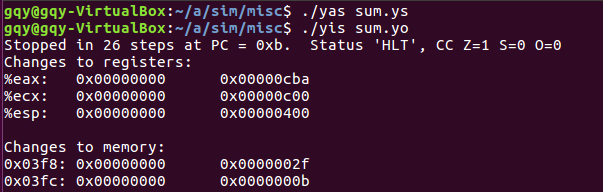
\includegraphics{A_sum}
		\caption{Part A  {\ttfamily sum.ys}} \label{Part A: sum.ys}%标题 自动编号 label标签
\end{figure}
\begin{figure}[htbp]%figure浮动体环境 [htbp]指定位置
		\centering%居中排版
		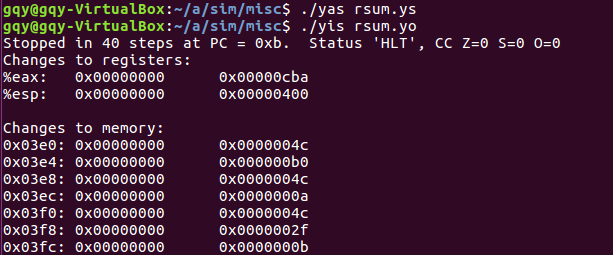
\includegraphics{A_rsum}
		\caption{Part A  {\ttfamily rsum.ys}} \label{Part A: rsum.ys}%标题 自动编号 label标签
\end{figure}
\begin{figure}[htbp]%figure浮动体环境 [htbp]指定位置
		\centering%居中排版
		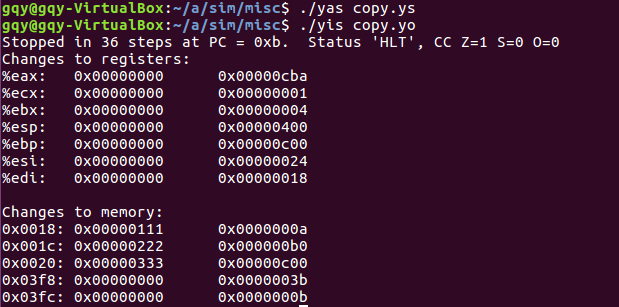
\includegraphics{A_copy}
		\caption{Part A  {\ttfamily copy.ys}} \label{Part A: copy.ys}%标题 自动编号 label标签
\end{figure}

\newpage
\subsection{Part B}

\subsubsection{Analysis}

In part B, we are asked to extend the SEQ processor to support instruction  {\ttfamily iaddl} and  {\ttfamily leave} by modifying file  {\ttfamily seq-full.hcl}. It’s important for this task to understand the implementation of HCL file and the data path of the two new instructions.\\

{\normalsize\bfseries Difficult point}
\begin{itemize}
\item[$\bullet$]Understand the processing logic and the syntax of HCL. 
\item[$\bullet$]Design the data path of the  {\ttfamily iaddl} instruction and the  {\ttfamily leave} instruction.
\end{itemize}
\noindent
The function of  {\ttfamily iaddl} is to add a constant value to a register. To achieve this, we should firstly use  {\ttfamily irmovl} to move the constant value to another register then use  {\ttfamily addl} to add the value to the destination register. The format of  {\ttfamily iaddl} is as below.\\
{\ttfamily iaddl C, rB\\rB = C + rB}\\
The instruction leave writes the value in top of stack register {\ttfamily \%ebp} to register {\ttfamily \%esp}. The format of it is as bellow. \\
{\ttfamily movl \%ebp, \%esp\\popl \%ebp}\\
We can translate this instruction into:\\
{\ttfamily \%ebp\_new = (\%esp\_odd)\\\%esp\_new = \%esp\_odd + 4}\\
The stage division of these two instructions is shown in the Table \ref{the stage division of iaddl and leave}.\\
\begin{table}[htbp]
\centering
\caption{the stage division of {\ttfamily iaddl} and {\ttfamily leave}}\label{the stage division of iaddl and leave}%标题
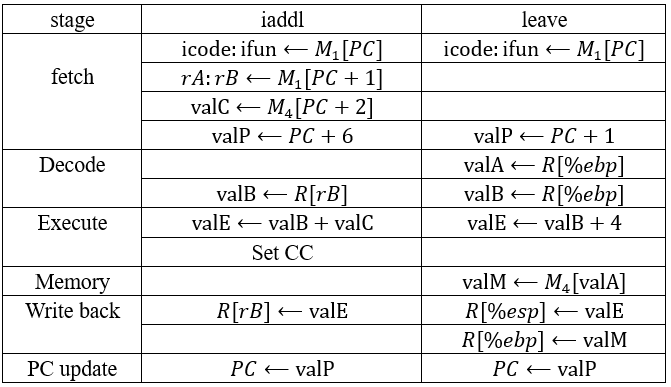
\includegraphics{stage}
\end{table}
\newpage
{\normalsize\bfseries Modify the {\ttfamily seq-full.hcl} file}
\begin{itemize}
\item[$\bullet$]Firstly, define ILEAVE as symbolic representation of leave instruction codes.
\item[$\bullet$]Add IIADDL and ILEAVE in the choice region instr\_valid to make them valid. 
\item[$\bullet$]Add IIADDL in the choice region of need\_regids since iaddl operation involves one register. The leave instruction doesn’t need it.
\item[$\bullet$]Add IIADDL in the choice region of need\_valC since iaddl operation need constant parameter. The leave instruction doesn’t need it.
\item[$\bullet$]When icode is ILEAVE, set the srcA as REBP. For iaddl, there is no need to set because the first operand of iaddl is not a register.
\item[$\bullet$]When icode is IIADDL, set the srcB as rB. When icode is ILEAVE, set the srcB as REBP.
\item[$\bullet$]When icode is IIADDL, set the dstE as rB. When icode is ILEAVE set the dstE as RESP. Because iaddl adds the immediate number into the destination register and leave writes value into register \%esp.
\item[$\bullet$]When icode is ILEAVE, set the dstM as REBP because we also need to update the value in register \%ebp. For IIADDL, there is no need to set.
\item[$\bullet$]When icode is IIADDL, set aluA as valC. When icode is ILEAVE, set aluA as 4. It’s the first operand of ALU.
\item[$\bullet$]When icode is IIADDL, set aluB as valB. When icode is ILEAVE, set aluB as valA. It’s the second operand of ALU.
\item[$\bullet$]When icode is IIADDL, alufun will be ALUADD since the operation is “adding”.
\item[$\bullet$]Add IIADDL in the choice region of set\_cc since iaddl operation involves ALU operation which will set flags. For leave, we don’t need it.
\item[$\bullet$]When icode is ILEAVE, set the control signal mem\_read. Instruction iaddl doesn’t need access to memory.
\item[$\bullet$]When icode is ILEAVE, set mem\_addr as valA. For iaddl, we don’t need it.
\end{itemize}
\subsubsection{Code}

\begin{center}
Modifications in {\ttfamily seq-full.hcl}
\end{center}
\begin{lstlisting}[language={[x86masm]Assembler}]
# 519021910095 QianyunGuo
# 519021910575 MuchenPan
-----------------------------------------------------------------------------------
# Instruction code for iaddl instruction
intsig IIADDL	'I_IADDL'
# Instruction code for leave instruction
intsig ILEAVE   'I_LEAVE'
-----------------------------------------------------------------------------------
################ Fetch Stage 
bool instr_valid = icode in 
	{ INOP, IHALT, IRRMOVL, IIRMOVL, IRMMOVL, IMRMOVL,
	       IOPL, IIADDL,IJXX, ICALL, IRET, IPUSHL, IPOPL, ILEAVE };
-----------------------------------------------------------------------------------
# Does fetched instruction require a regid byte?
bool need_regids =
	icode in { IRRMOVL, IOPL, IIADDL, IPUSHL, IPOPL, 
		     IIRMOVL, IRMMOVL, IMRMOVL };
-----------------------------------------------------------------------------------
# Does fetched instruction require a constant word?
bool need_valC =
	icode in { IIRMOVL, IIADDL, IRMMOVL, IMRMOVL, IJXX, ICALL };
-----------------------------------------------------------------------------------
################ Decode Stage
## What register should be used as the A source?
int srcA = [
	icode in { IRRMOVL, IRMMOVL, IOPL, IPUSHL  } : rA;
	icode in { IPOPL, IRET } : RESP;
        icode in { ILEAVE } : REBP;
	1 : RNONE; # Don't need register
];
-----------------------------------------------------------------------------------
## What register should be used as the B source?
int srcB = [
	icode in { IOPL, IIADDL, IRMMOVL, IMRMOVL  } : rB;
	icode in { IPUSHL, IPOPL, ICALL, IRET } : RESP;
        icode in { ILEAVE } : REBP;
	1 : RNONE;  # Don't need register
];
-----------------------------------------------------------------------------------
## What register should be used as the E destination?
int dstE = [
	icode in { IRRMOVL } && Cnd : rB;
	icode in { IIRMOVL, IOPL,IIADDL} : rB;
	icode in { IPUSHL, IPOPL, ICALL, IRET, ILEAVE } : RESP;
	1 : RNONE;  # Don't write any register
];
-----------------------------------------------------------------------------------
## What register should be used as the M destination?
int dstM = [
	icode in { IMRMOVL, IPOPL } : rA;
        icode in { ILEAVE } : REBP;
	1 : RNONE;  # Don't write any register
];
-----------------------------------------------------------------------------------
################ Execute Stage
## Select input A to ALU
int aluA = [
	icode in { IRRMOVL, IOPL } : valA;
	icode in { IIRMOVL, IRMMOVL, IMRMOVL, IIADDL } : valC;
	icode in { ICALL, IPUSHL } : -4;
	icode in { IRET, IPOPL, ILEAVE } : 4;
	# Other instructions don't need ALU
];
-----------------------------------------------------------------------------------
## Select input B to ALU
int aluB = [
	icode in { IRMMOVL, IMRMOVL, IOPL, IIADDL, ICALL, 
		      IPUSHL, IRET, IPOPL } : valB;
	icode in { IRRMOVL, IIRMOVL } : 0;
        icode in { ILEAVE } : valA;
	# Other instructions don't need ALU
];
-----------------------------------------------------------------------------------
## Set the ALU function
int alufun = [
	icode == IOPL : ifun;
        icode == IIADDL : ALUADD;
	1 : ALUADD;
];
-----------------------------------------------------------------------------------
## Should the condition codes be updated?
bool set_cc = icode in { IOPL,IIADDL };
-----------------------------------------------------------------------------------
################ Memory Stage
## Set read control signal
bool mem_read = icode in { IMRMOVL, IPOPL, IRET, ILEAVE };
-----------------------------------------------------------------------------------
## Select memory address
int mem_addr = [
	icode in { IRMMOVL, IPUSHL, ICALL, IMRMOVL } : valE;
	icode in { IPOPL, IRET, ILEAVE } : valA;
	# Other instructions don't need address
];
\end{lstlisting}

\subsubsection{Evaluation}

\begin{itemize}
\item[$\bullet$]Test the implementation on the Y86 benchmark programs in directory {\ttfamily y86-code}.  (Figure \ref{Part B: benchmark test})\\
The result shows the test on benchmark programs succeeded, so our simulator still correctly executess the benchmark suite.
\item[$\bullet$]Regression test (test everything except {\ttfamily iaddl} and {\ttfamily leave}) succeeded. (Figure \ref{Part B: regression test})
\item[$\bullet$]test {\ttfamily iaddl} (Figure \ref{Part B: ptest for iaddl}), test {\ttfamily leave} (Figure \ref{Part B: ptest for leave}), test {\ttfamily iaddl} and {\ttfamily leave} (Figure \ref{Part B: ptest for iaddl and leave}).\\
All the tests  succeeded.
\end{itemize}
\begin{figure}[htbp]%figure浮动体环境 [htbp]指定位置
		\centering%居中排版
		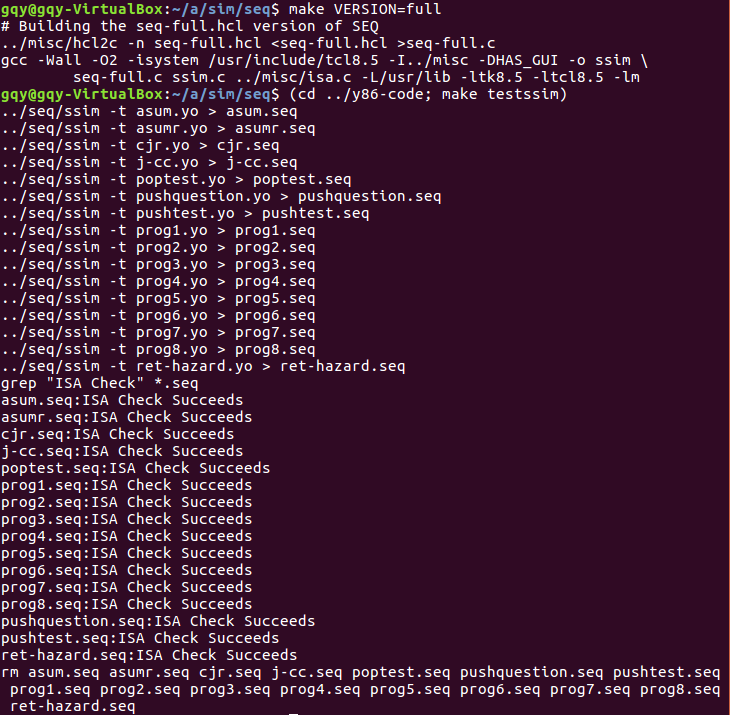
\includegraphics{B_benchmark}
		\caption{Part B benchmark test} \label{Part B: benchmark test}%标题 自动编号 label标签
\end{figure}
\begin{figure}[htbp]%figure浮动体环境 [htbp]指定位置
		\centering%居中排版
		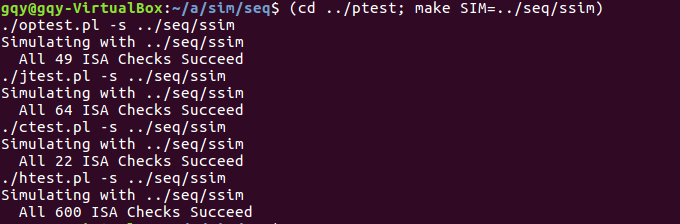
\includegraphics{B_regression}
		\caption{Part B regression test} \label{Part B: regression test}%标题 自动编号 label标签
\end{figure}
\begin{figure}[htbp]%figure浮动体环境 [htbp]指定位置
		\centering%居中排版
		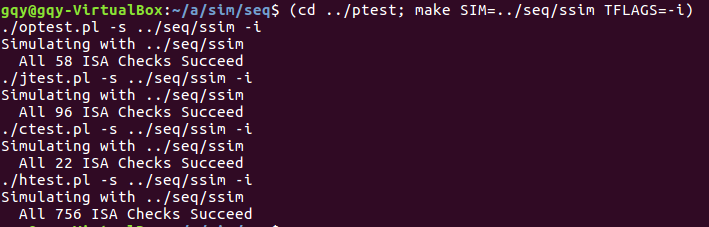
\includegraphics{B_ptesti}
		\caption{Part B ptest for {\ttfamily iaddl}} \label{Part B: ptest for iaddl}%标题 自动编号 label标签
\end{figure}
\begin{figure}[htbp]%figure浮动体环境 [htbp]指定位置
		\centering%居中排版
		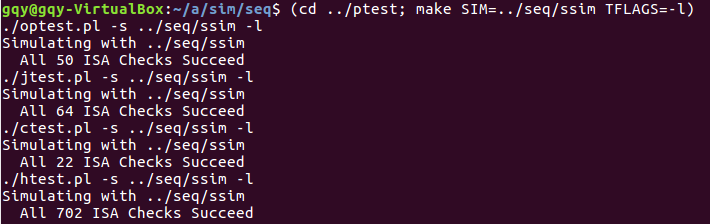
\includegraphics{B_ptestl}
		\caption{Part B ptest for {\ttfamily leave}} \label{Part B: ptest for leave}%标题 自动编号 label标签
\end{figure}
\begin{figure}[htbp]%figure浮动体环境 [htbp]指定位置
		\centering%居中排版
		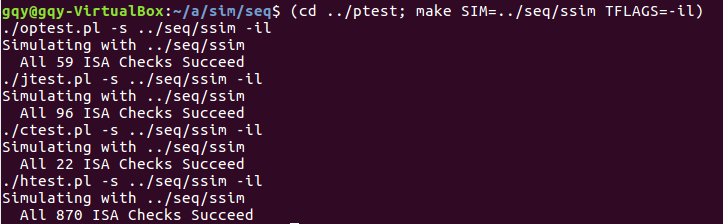
\includegraphics{B_ptestil}
		\caption{Part B ptest for {\ttfamily iaddl} and {\ttfamily leave}} \label{Part B: ptest for iaddl and leave}%标题 自动编号 label标签
\end{figure}

\newpage
\subsection{Part C}

\subsubsection{Analysis}
In this part, our task is to modify {\ttfamily ncopy.ys} and {\ttfamily pipe-full.hcl} with the goal of making {\ttfamily ncopy.ys} run as fast as possible.  \\

{\normalsize\bfseries Difficult point}
\begin{itemize}
\item[$\bullet$]Have a clear visage of the operation of pipelining according to the assembly language.
\item[$\bullet$]Find the extra overhead of the pipeline that we can avoid.
\item[$\bullet$]Explore proper ways to optimize the performance.
\item[$\bullet$]Implement all the proper ways with assembly language correctly.\\
\end{itemize}

{\normalsize\bfseries  Optimization steps}
\begin{itemize}
\item[$\bullet$]{\bfseries Add iaddl Instruction to {\ttfamily pipe-full.hcl}}\\
We extended the processor to support a new instruction: {\ttfamily iaddl} like what we have done in part B. In this way, we avoided extra steps to save a constant in a register. After optimizing the program by adding the instruction iaddl, our CPE test reached 13.96.
\item[$\bullet$]{\bfseries 4-Way Loop Unrolling}\\
Since predicting loops takes a lot of time, we choose to perform “loop unrolling” to minimize this overhead. “4-Way Loop Unrolling” is to do 4 loops each time and update the relevant data every 4 loops. When the length is less than 4, we change to the remaining part which is still in a loop way. In this way, our CPE test reached 11.28. Therefore, we can see “loop unrolling” is an efficient way for pipeline optimization.
\item[$\bullet$]{\bfseries 10-Way Loop Unrolling}\\
After 4-Way Loop Unrolling, we consider the more way we unroll the loops, the better performance we will have. So, we tried 10-Way Loop Unrolling and the implementation is the same as the last step. However, our CPE test only reached 11.21. Performance has improved, but not significantly.
\item[$\bullet$]{\bfseries Increase the Number of Registers}\\
We noticed that there exists stall between reading the val from the src and testing if the val is less than zero in each loop. After unrolling the loop, we can use two registers to store the val from src. So in each loop, the val we test has already been read in the last loop. In this way, our CPE test reached 10.51, which is a significant improvement. 
\item[$\bullet$]{\bfseries Combine 10-Way Loop Unrolling and 4-Way Loop Unrolling}\\
When taking CPE test, it can be seen that when the input is small, the performance of 10-way loop unrolling is not that useful. Thus, we have to optimize the remaining part. Taking the 4-way loop unrolling we tried before into account, we choose to change the remaining part to another loop unrolling. Fortunately, our CPE test reached 10.16.
\end{itemize}

\subsubsection{Code}

\begin{center}
Modifications in {\ttfamily pipe-full.hcl}
\end{center}
\begin{lstlisting}[language={[x86masm]Assembler}]
# 519021910095 QianyunGuo
# 519021910575 MuchenPan
#  We only added instruction iaddl here. The modifications are the same as what 
#we have done in Part B.
#  Define IIADDL as symbolic representation of leave instruction codes.
#  Add IIADDL in the choice region instr_valid to make them valid.
#  Add IIADDL in the choice region of need_regids since iaddl operation involves
#one register. 
#  Add IIADDL in the choice region of need_valC since iaddl operation need 
#constant parameter. 
#  Set the srcB as rB. 
#  Set the dstE as rB. Because iaddl adds the immediate number into the destination
#register and leave writes value into register %esp.
#  Set aluA as valC. It is the first operand of ALU.
#  Set aluB as valB. It is the second operand of ALU.
#  Add IIADDL in the choice region of set_cc since iaddl operation involves ALU 
#operation which will set flags.
-----------------------------------------------------------------------------------
# Instruction code for iaddl instruction
intsig IIADDL	'I_IADDL'
-----------------------------------------------------------------------------------
# Is instruction valid?
bool instr_valid = f_icode in 
	{ INOP, IHALT, IRRMOVL, IIRMOVL, IRMMOVL, IMRMOVL,
	  IOPL, IJXX, ICALL, IRET, IPUSHL, IPOPL, IIADDL };##
-----------------------------------------------------------------------------------
# Does fetched instruction require a regid byte?
bool need_regids =
	f_icode in { IRRMOVL, IOPL, IPUSHL, IPOPL, 
		     IIRMOVL, IRMMOVL, IMRMOVL, IIADDL };##
-----------------------------------------------------------------------------------
# Does fetched instruction require a constant word?
bool need_valC =
	f_icode in { IIRMOVL, IRMMOVL, IMRMOVL, IJXX, ICALL, IIADDL };##
-----------------------------------------------------------------------------------
## What register should be used as the B source?
int d_srcB = [
	D_icode in { IOPL, IRMMOVL, IMRMOVL, IIADDL  } : D_rB;##
	D_icode in { IPUSHL, IPOPL, ICALL, IRET } : RESP;
	1 : RNONE;  # Don't need register
];
-----------------------------------------------------------------------------------
## What register should be used as the E destination?
int d_dstE = [
	D_icode in { IRRMOVL, IIRMOVL, IOPL, IIADDL} : D_rB;##
	D_icode in { IPUSHL, IPOPL, ICALL, IRET } : RESP;
	1 : RNONE;  # Don't write any register
];
-----------------------------------------------------------------------------------
## Select input A to ALU
int aluA = [
	E_icode in { IRRMOVL, IOPL } : E_valA;
	E_icode in { IIRMOVL, IRMMOVL, IMRMOVL, IIADDL } : E_valC;##
	E_icode in { ICALL, IPUSHL } : -4;
	E_icode in { IRET, IPOPL } : 4;
	# Other instructions don't need ALU
];
-----------------------------------------------------------------------------------
## Select input B to ALU
int aluB = [
	E_icode in { IRMMOVL, IMRMOVL, IOPL, ICALL, 
		     IPUSHL, IRET, IPOPL, IIADDL } : E_valB;##
	E_icode in { IRRMOVL, IIRMOVL } : 0;
	# Other instructions don't need ALU
];
-----------------------------------------------------------------------------------
## Should the condition codes be updated?
bool set_cc = E_icode in { IOPL, IIADDL } &&
	# State changes only during normal operation
	!m_stat in { SADR, SINS, SHLT } && !W_stat in { SADR, SINS, SHLT };

\end{lstlisting}

\begin{center}
{\ttfamily ncopy-ys}
\end{center}
\begin{lstlisting}[language={[x86masm]Assembler}]
#/* $begin ncopy-ys */
##################################################################
# ncopy.ys - Copy a src block of len ints to dst.
# Return the number of positive ints (>0) contained in src.
#
# 519021910095 QianyunGuo
# 519021910575 MuchenPan
#
#  As our optimization steps in the Analysis section,our modifications of ncopy.ys
#are as follows.

#######Add iaddl###################################
#  Use iaddl to avoid using a register to save a constant while changing the value
#in a register like count++, len--, src++ and so on.

#######Loop unrolling. Combine 10-way and 4-way##############
#  First, we enter 10-way loop unrolling part.
#  We test whether len (%edx) is less than 10
#  If so, go to Remainloop part which is 4-way loop unrolling
#  Otherwise, we loop 10 times and in the end we enter Npos10 part in which we
#update the data of src (%ebx) and dst (%ecx) and test whether len (%edx) is less
#than 10 again to choose whether take another 10-way loop.

#  The 4-way loop unrolling in the Remainloop part is the same as 10-way loop.
#  We test whether len (%edx) is less than 4
#  If so, go to Remain part which is traditional loop part.
#  Otherwise, we loop 4 times and in the end we enter Npos4 part in which we
#update the data of src (%ebx) and dst (%ecx) and test whether len (%edx) is less
#than 4 again to choose whether take another 4-way loop.

#  Last part is Remain, a traditional loop part. We update the data of src (%ebx) 
#and dst (%ecx) and test len (%edx) in every loop.

#######Increase the Number of Registers#####################
#  Two registers (%esi and %edi) are used alternately for each loop section. 
#  In every loop, one store the current val and the other read the val we need to
#test in the next loop. Also, we changed instruction order when necessary.

##################################################################
# Do not modify this portion
# Function prologue.
ncopy:	pushl %ebp		# Save old frame pointer
	rrmovl %esp,%ebp	# Set up new frame pointer
	pushl %esi		# Save callee-save regs
	pushl %ebx
	pushl %edi
	mrmovl 8(%ebp),%ebx	# src
	mrmovl 16(%ebp),%edx	# len
	mrmovl 12(%ebp),%ecx	# dst

##################################################################
# You can modify this portion
	# Loop header
	iaddl $-10, %edx	# len -=10;
	xorl %eax,%eax		# count = 0;
	andl %edx,%edx		# len <= 0?
	jle Remainloop		# if len <= 0, goto Remainloop:

Loop0:	
	mrmovl (%ebx), %esi	# read val from src
	mrmovl 4(%ebx),%edi	# read next val from next src
	andl %esi, %esi		# current val <= 0?
	rmmovl %esi, (%ecx)	# store current val to dst
	jle Loop1		# if so, goto Loop1:
	iaddl $1, %eax		# count++
Loop1:	
	mrmovl 8(%ebx), %esi	# read next val from next src
	andl %edi, %edi		# current val <= 0?
	rmmovl %edi, 4(%ecx)	# store current val to dst
	jle Loop2		# if so, goto Loop2:
	iaddl $1, %eax		# count++
Loop2:	
	mrmovl 12(%ebx), %edi	# read next val from next src
	andl %esi, %esi		# current val <= 0?
	rmmovl %esi, 8(%ecx)	# store current val to dst
	jle Loop3		# if so, goto Loop3:
	iaddl $1, %eax		# count++
Loop3:	
	mrmovl 16(%ebx), %esi	# read next val from next src
	andl %edi, %edi		# current val <= 0?
	rmmovl %edi, 12(%ecx)	# store current val to dst
	jle Loop4		# if so, goto Loop4:
	iaddl $1, %eax		# count++
Loop4:	
	mrmovl 20(%ebx), %edi	# read next val from next src
	andl %esi, %esi		# current val <= 0?
	rmmovl %esi, 16(%ecx)	# store current val to dst
	jle Loop5		# if so, goto Loop5:
	iaddl $1, %eax		# count++
Loop5:	
	mrmovl 24(%ebx), %esi	# read next val from next src
	andl %edi, %edi		# current val <= 0?
	rmmovl %edi, 20(%ecx)	# store current val to dst
	jle Loop6		# if so, goto Loop6:
	iaddl $1, %eax		# count++
Loop6:	
	mrmovl 28(%ebx), %edi	# read next val from next src
	andl %esi, %esi		#current val <= 0?
	rmmovl %esi, 24(%ecx)	# store current val to dst
	jle Loop7		# if so, goto Loop7:
	iaddl $1, %eax		# count++
Loop7:	
	mrmovl 32(%ebx), %esi	# read next val from next src
	andl %edi, %edi		# current val <= 0?
	rmmovl %edi, 28(%ecx)	# store current val to dst
	jle Loop8		# if so, goto Loop8:
	iaddl $1, %eax		# count++
Loop8:	
	mrmovl 36(%ebx), %edi	# read next val from next src
	andl %esi, %esi		# current val <= 0?
	rmmovl %esi, 32(%ecx)	# store current val to dst
	jle Loop9		# if so, goto Loop9:
	iaddl $1, %eax		# count++
Loop9:	
	andl %edi, %edi		# val <= 0?
	rmmovl %edi, 36(%ecx)	# store current val to dst
	jle Npos10		# if so, goto Npos10:
	iaddl $1, %eax		# count++
Npos10:	
	iaddl $-10, %edx	# len-10
	iaddl $40, %ebx		# src+10
	iaddl $40, %ecx		# dst+10
	andl %edx,%edx		# len > 0?
	jg Loop0		# if so, goto Loop0:
#######################
Remainloop:
	iaddl $6, %edx		# len +=6;
	andl %edx,%edx		# len <= 0?
	jle Remain		# if so, goto Remain:

Loop40:	
	mrmovl (%ebx), %esi	# read val from src...
	mrmovl 4(%ebx),%edi	# read next val from next src
	andl %esi, %esi		# val <= 0?
	rmmovl %esi, (%ecx)	# store current val to dst
	jle Loop41		# if so, goto Loop41:
	iaddl $1, %eax		# count++
Loop41:	
	mrmovl 8(%ebx), %esi	# read next val from next src
	andl %edi, %edi		# val <= 0?
	rmmovl %edi, 4(%ecx)	# store current val to dst
	jle Loop42		# if so, goto Loop42:
	iaddl $1, %eax		# count++
Loop42:	
	mrmovl 12(%ebx), %edi	# read next val from next src
	andl %esi, %esi		# val <= 0?
	rmmovl %esi, 8(%ecx)	# store current val to dst
	jle Loop43		# if so, goto Loop43:
	iaddl $1, %eax		# count++
Loop43:	
	andl %edi, %edi		# val <= 0?
	rmmovl %edi, 12(%ecx)	# store current val to dst
	jle Npos4		# if so, goto Npos4:
	iaddl $1, %eax		# count++
Npos4:	
	iaddl $-4, %edx		# len-=4;
	iaddl $16, %ebx		# src+=4;
	iaddl $16, %ecx		# dst+=4;
	andl %edx,%edx		# len > 0?
	jg Loop40		# if so, goto Loop40:

Remain:
	iaddl $4, %edx		# len+=4;
	andl %edx, %edx		# len <= 0?
	jle Done		# if so, goto Done:
Loop:
	mrmovl (%ebx), %esi	# read val from src...
	rmmovl %esi, (%ecx)	# ...and store it to dst
	andl %esi, %esi		# val <= 0?
	jle RemNpos		# if so, goto RemNpos:
	iaddl $1, %eax		# count++
RemNpos:
	iaddl $-1, %edx		# len--
	iaddl $4, %ebx		# src++
	iaddl $4, %ecx		# dst++
	andl %edx,%edx		# len > 0?
	jg Loop			# if so, goto Loop:

	
##################################################################
# Do not modify the following section of code
# Function epilogue.
Done:
	popl %edi               # Restore callee-save registers
	popl %ebx
	popl %esi
	rrmovl %ebp, %esp
	popl %ebp
	ret
##################################################################
# Keep the following label at the end of your function
End:
#/* $end ncopy-ys */

\end{lstlisting}


\subsubsection{Evaluation}

\begin{itemize}
\item[$\bullet$]Y86 benchmark test in directory {\ttfamily y86-code} succeeded (Figure \ref{Part C: benchmark test}).
\item[$\bullet$]Regression test with {\ttfamily iaddl} test succeeded (Figure \ref{Part C: ptest with iaddl}).
\item[$\bullet$]Correctness test succeeded (Figure \ref{Part C: Correctness test}). 
\item[$\bullet$]CPE test(Figure \ref{Part C: CPE test}). Our average CPE is 10.16 and we score 56.1.
\end{itemize}
\begin{figure}[htbp]%figure浮动体环境 [htbp]指定位置
		\centering%居中排版
		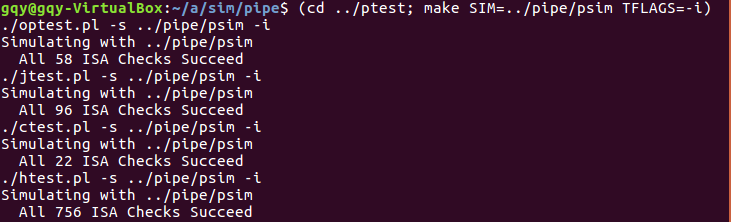
\includegraphics{C_ptesti}
		\caption{Part C ptest with {\ttfamily iaddl}} \label{Part C: ptest with iaddl}%标题 自动编号 label标签
\end{figure}
\begin{figure}[htbp]%figure浮动体环境 [htbp]指定位置
		\centering%居中排版
		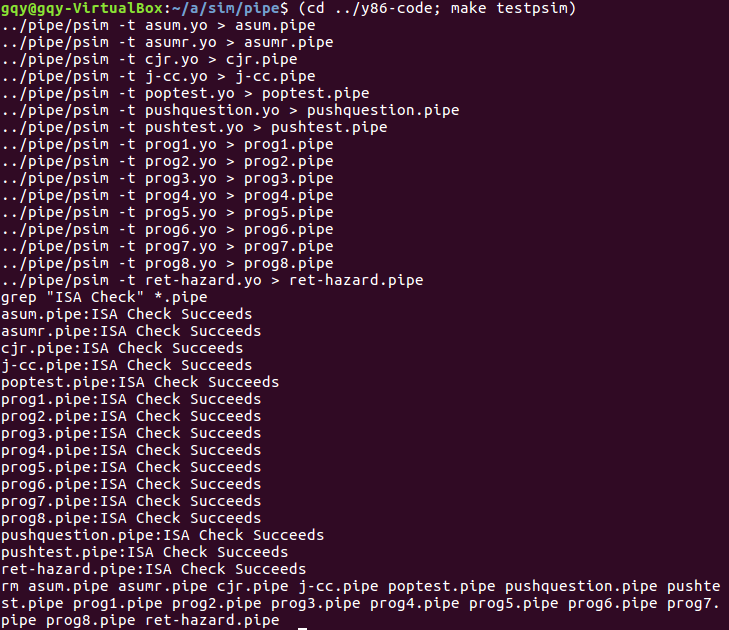
\includegraphics{C_benchmark}
		\caption{Part C benchmark test} \label{Part C: benchmark test}%标题 自动编号 label标签
\end{figure}
\begin{figure}[htbp]
\centering
\subfigure[Part C Correctness test]{
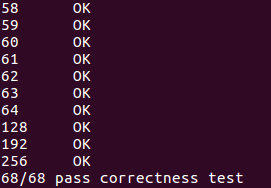
\includegraphics{C_correctness}\label{Part C: Correctness test}
}
\quad
\subfigure[Part C CPE test]{
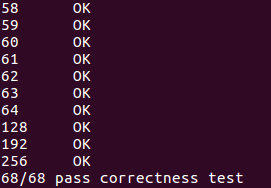
\includegraphics{C_correctness}\label{Part C: CPE test}
}
\caption{Part C correctness and CPE test}
\end{figure}

\newpage
\section{Conclusion}
\subsection{Problems}
\begin{itemize}
\item[$\bullet$]Get familiar with new language and tools. Since Y86 assembly language is s new language for us. Before we start out project, we have to learn about the basic language knowledge including gramma and instruction meaning.
\item[$\bullet$]Take care of the use of stack, registers, and variables. Assembly language operate on registers and memory directly, so it is critical to take care of all these.
\item[$\bullet$]Get the meaning of new instruction and figure out how to implement it. In the process we learned from CS:APP to further explore the instruction implementation.
\item[$\bullet$]Analyze the pipeline performance and relevant factors. Explore and design proper ways to optimize it. As our optimize process described in Part C is not a smooth ride, and in the end we did not score a full mark in CPE test. It shows that our pipeline still has room for optimization. If there is an opportunity, we will continue to explore different ways to optimize pipeline performance.
\end{itemize}

\subsection{Achievements}
In this project, our group successfully completed the three part.
\begin{itemize}
\item[$\bullet$] In Part A, we transferred three functions about linked list in example.c into Y86 code with the basic knowledge of the Y86 assembly language. 
\item[$\bullet$] In Part B, we added the iaddl instruction and the leave instruction to Y86’s sequential design by modifying the HCL file after a deep exploring into the stages of these two instructions. 
\item[$\bullet$] In Part C, we improved and optimized the performance of the pipeline processor with proper ways including adding instructions, using loop unrolling, adding registers and changing the instruction order.
\item[$\bullet$] Take care of the readability of our codes. Assembly language is less readable than high-level language, so we added detailed comments in our codes. Also, our optimization method is described in detail.
\item[$\bullet$] In the process of the project, both two group members all made contributions to the project and report part, which is a good cooperation. Besides, we both have found it a very interesting and meaningful project which helped us know better about the implementation of a pipelined Y86 processor. 
\end{itemize}
Finally, we would like to appreciate Miss Shen and teaching assistants for their careful guidance and support, from which we have benefited a lot.



%----------------------------------------------------------------------------------------


\end{document}